\documentclass[12pt,letterpaper,titlepage]{article}

\usepackage{fontspec}
\defaultfontfeatures{Mapping=tex-text}
\usepackage{xunicode}
\usepackage{xltxtra}
\usepackage{amsmath}
\usepackage{pdfpages}
\usepackage{amsfonts}
\usepackage{amssymb}
\setcounter{secnumdepth}{0}
\usepackage{nameref}
\usepackage{enumitem}
\usepackage{environ}
\usepackage{pgfplots}

\setmainfont{Times New Roman}
\showboxdepth=\maxdimen
\showboxbreadth=\maxdimen


\usepackage{paracol}
\usepackage{wrapfig}
\globalcounter{table}
\globalcounter{figure}
\usepackage{graphicx}
\usepackage[left=1in,right=1in,top=1in,bottom=1in]{geometry}
\graphicspath{{img/}}

\author{Jacob Abel}
\title{	Design \& Simulate 1 Ex1.2
	\\\large ECE2204 CRN:82929
}

\setlength{\parskip}{0.5em}

\begin{document}
\maketitle
\begin{raggedright}

\section{Problem 1.2.a.1: }
\subsection{Design}

Consider silicon at $T = 350K$ doped with boron at an unknown concentration. The electron concentration is $n_o = 7.3 \times 10^5 cm^{-3}$. Silicon's bandgap energy is $E_g = 1.1eV$ and Silicon's semiconductor constant is $B = 5.23 \times 10^{15} cm^{-3}K^{\frac{-3}{2}}$. Determine the acceptor concentration $N_a$.

\begin{equation}\scalebox{1.25}{
$
n_i = BT^{\frac{3}{2}}e^{(\frac{-E_g}{2kT})} 
$
}
\end{equation}
\begin{equation}\scalebox{1.25}{
$
n_i = (5.23\times 10^{15})(350)^{\frac{3}{2}}e^{
	\big(\frac{-1.1}{
		2(86\times 10^{-6})(350)
	}\big)
	} 
	= 3.97\times 10^{11} cm^{-3}
$
}
\end{equation}
	
\begin{equation}\scalebox{1.25}{
$
p_o = \frac{n_i^2}{n_o} 
	= \frac{
	(3.97\times 10^{11} cm^{-3})^2
}{
	7.3 \times 10^5 cm^{-3}
}
	= 2.159 \times 10^{17} cm^{-3}
$
}
\end{equation}

As $p_o \gg n_i$, the acceptor concentration $N_a \approx p_o = 2.159 \times 10^{17} cm^{-3}$.

\pagebreak
\subsection{Validation}

\begin{center}
Mathematica Implementation (accurate with $< 1\%$ deviation from design result)
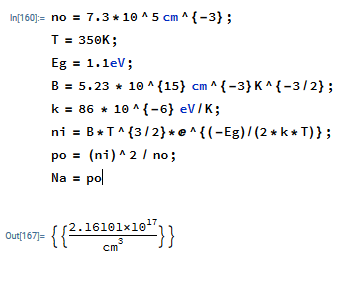
\includegraphics[width=.5\textwidth, height=\textheight, keepaspectratio=true]{ds1a}
\end{center}

\begin{center}
LTSpice Implementation (accurate with $< 1\%$ deviation from design result)
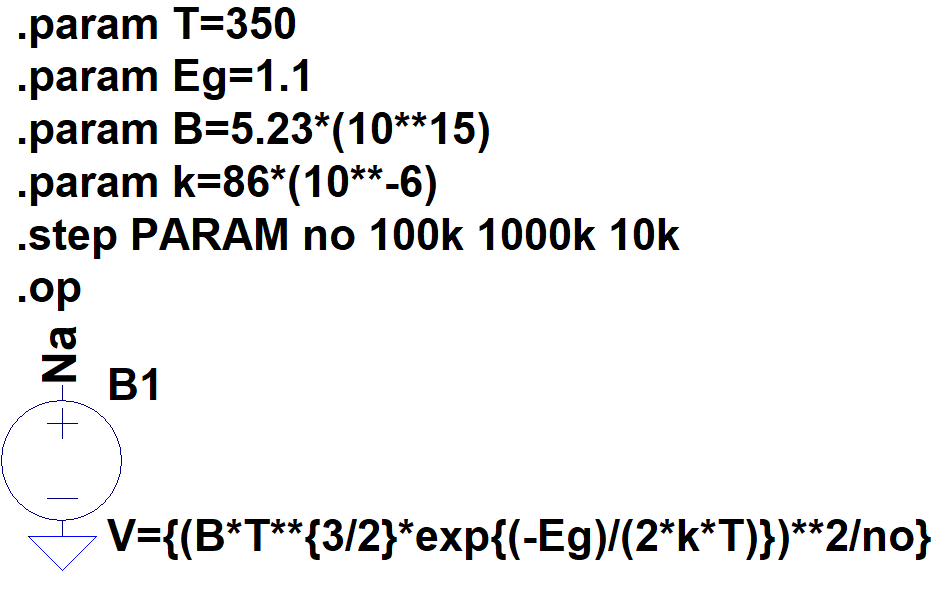
\includegraphics[width=.4\textwidth, height=\textheight, keepaspectratio=true]{ds1b}
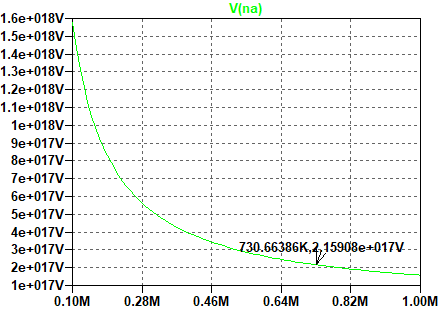
\includegraphics[width=.4\textwidth, height=\textheight, keepaspectratio=true]{ds1c}
\end{center}

\clearpage
\section{Problem 1.2.b.1: }
\subsection{Design}
Find the concentration of electrons and holes in a sample of germanium
that has a concentration of donor atoms equal to $N_d = 0.4 \times 10^{15} cm^{−3}$. Is the semiconductor n-type or p-type? Germanium's bandgap is $E_g = 0.66eV$ and its semiconductor constant is $B = 1.66 \times 10^{15} cm^{-3}K^{\frac{-3}{2}}$. The temperature is $T = 300K$

\begin{equation}\scalebox{1.25}{
$
n_i = (1.66\times 10^{15})(300)^{\frac{3}{2}}e^{
	\big(\frac{-0.66}{
		2(86\times 10^{-6})(300)
	}\big)
	} 
	= 2.40\times 10^{13} cm^{-3}
$
}
\end{equation}

As $N_d \gg n_i$, the electron concentration is $n_o \approx N_d = 0.4 \times 10^{15} cm^{-3}$.


\begin{equation}\scalebox{1.25}{
$
p_o	= \frac{
	(2.40\times 10^{13} cm^{-3})^2
}{
	0.4 \times 10^{15} cm^{-3}
}
	= 1.44 \times 10^{12} cm^{-3}
$
}
\end{equation}

The hole concentration $p_o = 1.44 \times 10^{12} cm^{-3}$. As the semiconductor has donor atoms, it is n-type.

\pagebreak
\subsection{Validation}

\begin{center}
Mathematica Implementation (accurate with $< 1\%$ deviation from design result)
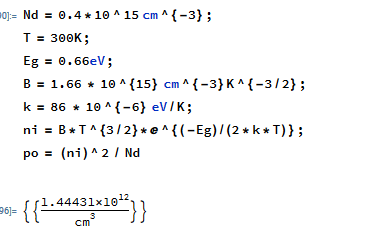
\includegraphics[width=.5\textwidth, height=\textheight, keepaspectratio=true]{ds2a}
\end{center}

\begin{center}
LTSpice Implementation (accurate with $< 1\%$ deviation from design result)
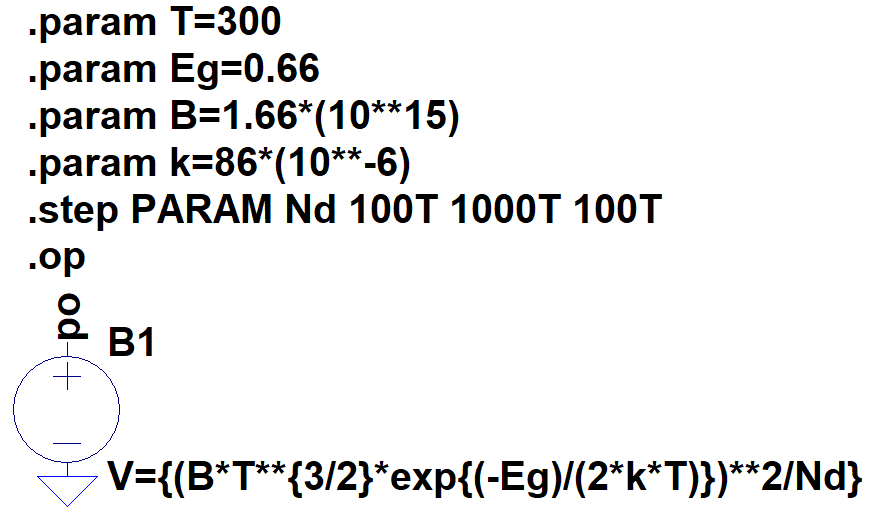
\includegraphics[width=.4\textwidth, height=\textheight, keepaspectratio=true]{ds2b}
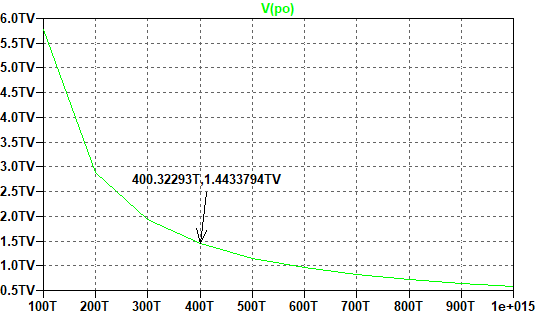
\includegraphics[width=.4\textwidth, height=\textheight, keepaspectratio=true]{ds2c}
\end{center}

\textit{I have neither given nor received unauthorized assistance on this assignment.}


\end{raggedright}
\end{document}
